\pagestyle{plain} \pagenumbering{arabic}

\begin{center}
{\Large{\bf \mytitle}}
\end{center}
\vspace{-0.1in}

\Section{Introduction}
\label{sec:intro}

Computer vision has been the subject of `humane care': Over the course of past several decades, the field of computer vision has been preoccupied with the enthusiasms of looking at humans. We detect the existences of faces and bodies in images, we track the detected human beings in videos, we recognize them, we estimate their poses, we interpret their behaviors and predict their activities, and we infer the scene, the geo-location, as well as the moment at which the human beings reside. The continuous efforts on studying humans via exhaustively exploiting visual information, and all remarkable progress we have achieved, are actually not surprising: it simply reflects the central role that the sense of sight plays in perception, especially the perception about ourselves. Images can convey a \emph{thousand} words" in the blink of an eye, and we are doing nothing but working toward intelligent machines that can reconstruct from images and videos as many words among the "thousand words" as possible.

Regardless of how many among the "thousand words" we can proudly claim to be already reconstructible from images and videos or under our current focus, we are now assuring you that we may actually have more untouched words about humans embedded in our visual media. Before we formally unveil the seemingly mysterious realm of untouched, let us first invite you to this simple and thought-provoking example, as shown in Fig. \ref{fig:intro} where two faces are detected from a image using methods such as \cite{ViolaJones} (a-1), and we expect to reveal whether the two individuals are friends, family members, or workmates. Immediately from the two detections we may compute the relative positions of the two faces (a-2), which however has little implication about the social relationship. After we go on to extract other visual descriptions such as expressions (a-3) using methods introduced in \cite{delaTorre:expression},  mutual gazes (a-4) using methods summarized in \cite{Hanson}, and mutual poses (a-5) using methods such as \cite{poselet}, we tend to believe the two individuals are not workmates. Finally, we may even recognize the background using scene analysis approach such as \cite{scene} by which we eventually are confident of a `friend' relationship between the two . 

The example is inspiring, in that it convinces us that we are equipped with sufficient image understanding capabilities, and a smart selection and leveraging of them reveals new `words' that has never been seen by computer vision.  It is also evident, that the realm of untouched words, which has been largely supported by contemporary computer vision functionalities but has received scarce attention, if not none, is the \emph{social} aspect of human beings. We foresee the time when we may visually \emph{sense} the human society, using ubiquitous visual information and cutting-edge computer vision technologies to estimate social relationships and attributes in various social networks. The rich social semantics embedded in visual media is actually not at all a misery, as we are fully aware that human beings are in a society and they are interrelated within social networks, and if we could have had realized this fact and brought social perspectives into computer vision earlier. We believe it the time to introduce computer vision to social sensing, and to begin advancing computer vision into a social-oriented age, from the present research where human beings are mostly treated as independent agents, and where social network research has hardly built upon pixels even though the studied online communities have been full of billions of images describing their members.

The lack of visual sensors in exploring social communities, on the other hand, is accompanied by the lack of social assistance in improving vision functionalities.  The fact that social contexts may have immeasurable potentials in pushing traditionally hard vision problems onto a new level is evident, for example, in the following task on face recognition from online imageries. Consider that we employ a state-of-art face recognizer to identify the two faces detected in Fig. \ref{fig:intro} (a-1), where the right face is hard to distinguish between `Susan' and `Helen' (see (b-1)). However, the social relationship as inferred from various visual features in (a-2) to (a-6) suggest that the individual should belong to the left person's close friends (see (b-2)), and there is eventually not a friend of `Mary' named `Susan'. Consequently, we gain significantly stronger confidence about the face hard to be recognized by a conventional recognizer. 

The success of such socially-assisted face recognition is credited to the textual metadata that has been manually attached to the imagery under investigation, and such manual tagging has been fully enabled and abundantly available in almost every online community, including major visually-centralized communities such as Flickr, YouTube, and Facebook where vision researchers harvest samples.  Recognizing a face can benefit from knowing about other faces appearing in the same picture or video: The fact is too obvious to be harnessed by the majority of face recognition research where a face is nothing but an isolated face and a million faces are simply a million such independent faces. The stories are in no ways limited to face recognition, because parsing humans' behaviors in videos can also draw input from their social relationships, inferring the scene in an image can leverage clues from other images co-existing in the same online album, and forecasting the event to show in a dome camera will become more accurate once we learn the patterns of social interactions under its surveillance from the volumes of prior recordings. Despite all these observations, contemporary computer vision treats images and videos as independent samples even if the scale of these sample sets has reached up to billion.

\begin{figure}[t!]
\begin{center}
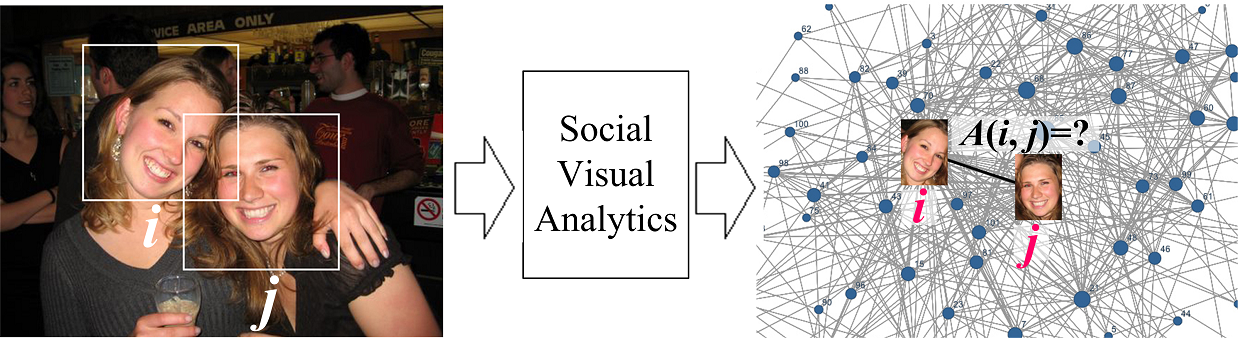
\includegraphics[width=\columnwidth]{intro}
\end{center}
\vspace{-0.25in} \caption{\captionsize 
(a-1) Original picture with detected faces; (a-2) relative positions of the detections; (a-3) Facial expressions; (a-4) Mutual Gazes; (a-5) Mutual poses; (a-6) scene recognition. (b-1) Independently recognizing the two faces: The right face is hard to distinguish between two possible people; (b-2) Recognizing faces using social relationship inferred from (a-1) through (a-6): The right face is now more likely to be associated with one person than the other. \label{fig:intro}\afterfigspace}
\end{figure}

Why do we believe that the approach of social sensing from visual information will be productive? It is because visual information exhibits its unique merits in reflecting the social semantics captured by cameras and depicted in the formats of images and videos. First, visual media from abundant online photos to video volumes harvested by surveillance camera networks are prevalent, and informative data is produced in a quantity thousand times of what conventional sensors do. Second, camera, as a new social sensor, is much less intrusive than conventional social sensors, but exposes us the `real stories' about the community members from aside and remotely: Many of these stories may be too subtle for conventional approaches to grasp but visually sensible. Third,  computer vision capabilities, as illustrated in the previous example, has supported a substantial necessary requirements for interpreting social relationship and attributes. In companion, we advocate the approach of visual understanding using social context, not only because `socially-incentivized' metadata, as afore-mentioned, has become mostly available to the networked imagery to which computer vision are devoting its attention, but also because these metadata and socially-oriented mechanisms have been adopted as the organizing and managing infrastructure. In other words, the pixels have been socialized, even though we have hardly exploited it, and are now bringing it onto agenda. Last but not least, both the approach of social sensing from visual information and the approach of visual understanding using social context will profit from a diversity of disciplines spanning sociology, pedagogy, statistics, and so on, and be enriched with the new concepts, perspectives, and approaches therein.

We propose a new paradigm, which we refer to as "\emph{socially-aware visual analytics}", to exploit the scarcely touched middle ground between computer vision and social networks, and to provide a foundation for such socially-aware computer vision systems. "Socially-aware" are two-fold: The awareness of vision by social networks and the awareness of social networks by vision, and in paralleling the two related lines of efforts, our goal is to enable the next generation of technology to both computer vision and social networks to maximally benefit from each other.  More Specifically, the two parts of our proposed activity include 
\begin{enumerate}
\item \vspace{-0.05in}\emph{Social sensing from visual information.} To transform visual cues into social semantics, we will first develop socially-informative representations of humans in images and videos. Specifically, these include human and behavior descriptors for gaze, expression, gesture, and pose in socialized environment. We will then develop learning mechanisms by which we detect and recognize interactions from still images and image sequence, and by which we aggregate inter-person relationships from short-term observations of these interactions as well as long term observations of their co-occurrence/co-ordination in a socialized scene. We will, in particular, account for the problem of learning and inference on large-scale graphs under realistic network conditions. These conditions include substantial unobservable nodes and links, multiple overlapping communities, and multiple heterogeneous attributes, which are hardly addressed even in contemporary social network research. In addition, we aim to establish a framework by which visually estimated networks are fused with and adapted to networks arising from other types of cues.
\item \vspace{-0.05in}\emph{Visual understanding using social context.} Building on our previous expertise, we will provide an unified generalized solution for face recognition under social context. our preliminary prototype has limited capability in handling realistic network conditions, such as unobservable and noisy nodes and links, multiple overlapping communities, and multi-view attributes. Our generalization is aimed to accounting for all these challenges and pursuing robust recognition in realistic applications. The solution will be also applicable to collective classification of an image set, such as an online image corpus or album, whose socially-incentivized meta-tags will thereby play their "social roles". We will also extend the usage of social context into video understanding, where the parsing of humans' group activity will receive guidance from sociological studies.
\item \vspace{-0.05in}\emph{Integrated Socially-Aware Computer Vision.} An overall socially-aware visual analytical system is our ultimate goal. To this end, our proposed research will include an attempt for a framework that eventually integrate social information and image understanding and allow them to learn self-build themselves in an evolving and unsupervised manner.
\end{enumerate}
We reiterate, at this moment when either of the two parts can develop broad and far in its own pace, that the visual sensing of a social network and the socially assisted visual understanding are closely related and both may benefit from cross-pollination: Visually sensed social ties provide more specific contextual evidences about who are more likely to interact in a new visual scene and what activities they are more likely to be engaged in, while watching the visual co-occurrences and co-activities of two community members may reflect more accurate connections between them that are not easily available from other resources. Our proposed activity considers the two complementing modules in a systematic and integrated manner, and allow a "co-computation" model allowing intermediate results being shared between them. 

Though the focus of the proposed research is online and networked visual media about humans, the tools we plan to develop will have much broader impact.  It will be also useful for other types of visual materials involving other than humans, such as historical image archives, scientific image collections, biological recordings, and so on. Socialized behaviors are prevalent in social creatures, and our research will shed lights on new approaches to automatic browse, index, and parse them. New insights will be drawn toward diverse disciplines spanning sociology, pedagogy, and statistics, which are still in their infancy in introducing automated approaches exploiting visual information. Besides the tremendous potentials of industrial interests and product implementation that do not need elaboration, the proposed interdisciplinary research will also prompt revolutions in educational programs providing next-generation students with more comprehensive knowledge and broader mastery of skills.